\title{The SVD and the Spectral Decomposition of a Matrix}
\subtitle{\SubTitleName}
\institute[]{\Course}
\author{\Instructor}
\maketitle   


\frame{\frametitle{Topics and Objectives}
\Emph{Topics} \\
%\TopicStatement
\begin{itemize}

    \item the Singular Value Decomposition (SVD) of a matrix and the spectral decomposition

\end{itemize}

\vspace{0.5cm}

\Emph{Learning Objectives}\\

%\LearningObjectiveStatement

\begin{itemize}

    % \item compute the SVD for a rectangular matrix
    \item apply the SVD to construct a spectral decomposition of a matrix
    % \end{itemize}
\end{itemize}

} 

\begin{frame}\frametitle{Motivation: Approximation}

    Recall that from calculus, Taylor expansions and Taylor polynomials, can be used to approximate functions near a point.
    \pause 
    \begin{center}
    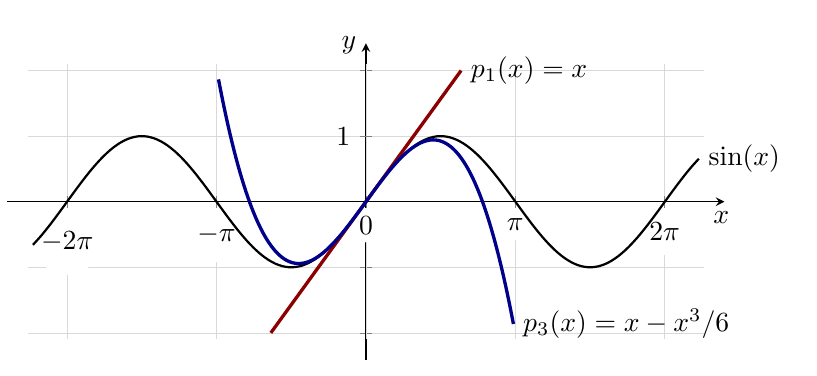
\begin{tikzpicture}[domain=-8:7] 
        \begin{axis}[
        width=4in,
        height=2.0in,
        grid=both,
        grid style={line width=.2pt, draw=gray!30},
        clip=false,
        axis lines=middle,
        xmin=-7.1,xmax=7.1,
        ymin=-2.1,ymax=2.1,
        restrict y to domain=-2:4,
        xtick={-6.28,-3.14,0,3.14,6.28},
        xticklabels={, , , , , , , , , ,},
        ytick={-2,-1,0,1,2},
        yticklabels={, , , , , , , , , ,},
        extra x ticks={-6.28,-3.14,0,3.14,6.28},
        extra y ticks={1},
        extra x tick style={xticklabel style={fill=white, circle, inner sep=1.5pt}},
        extra y tick style={xticklabel style={fill=white, circle, inner sep=1.5pt}},
        extra x tick labels={$-2\pi$, $-\pi$,$0$, $\pi$,$2\pi$},
        extra y tick labels={1},
        axis line style={shorten >=-7.5pt, shorten <=-7.5pt},
        xlabel=$x$,
        ylabel=$y$,
        xlabel style={at={(ticklabel* cs:1)},anchor=north west},
        ylabel style={at={(ticklabel* cs:1)},anchor=south east}
        ]
        
        \addplot[samples=100,domain=-7:7,smooth, thick] {sin(deg(x))} node[pos=1] (endofplotsquare) {};
        \node [right] at (endofplotsquare) {$\sin(x)$};  
        
        \addplot[samples=100,domain=-2:2,smooth, very thick,DarkRed] {x} node[pos=1] (endofplotsquare) {};
        \node [right] at (endofplotsquare) {$p_1(x)=x$};
        
        \addplot[samples=100,domain=-3.1:3.1,smooth, very thick,DarkBlue] {x-x*x*x/6} node[pos=1] (endofplotsquare) {};
        \node [right] at (endofplotsquare) {$p_3(x)=x-x^3/6$};           
        \end{axis}

    \end{tikzpicture}   
    \end{center}
    \pause Students are not expected to be familiar with Taylor expansions in this course, but, can we use expansions to approximate matrices? 
\end{frame}


\begin{frame}\frametitle{Recall: Spectral Decomposition of a Symmetric Matrix}

    \begin{center}\begin{tikzpicture} \node [mybox](box){\begin{minipage}{0.75\textwidth}\vspace{4pt}
        Suppose $A$ can be orthogonally diagonalized as 
        \begin{equation*}
        A = P D P ^{T} = \begin{pmatrix}
        \vec u_1 & \cdots & \vec u_n 
        \end{pmatrix}
        \begin{pmatrix}
            \lambda _1 & \cdots & 0 
            \\
            \vdots & \ddots &  \vdots
            \\
            0 & \cdots & \lambda _n 
        \end{pmatrix}
        \begin{pmatrix}
            \vec u_1  ^{T}  \\ \vdots \\ \vec u_n  ^{T} 
        \end{pmatrix}
        \end{equation*}
        Then $A$ has the decomposition
        $$A = 
        \lambda _1 \vec u_1 \vec u_1 ^{T}  + \cdots + \lambda _n \vec u_n \vec u_n ^{T} 
        = \sum_{i=1}^{n} \lambda_i \vec u_i \vec u_i^T$$
        \end{minipage}};
    \node[fancytitle, right=10pt] at (box.north west) {Spectral Decomposition};
    \end{tikzpicture}\end{center}
    
    \pause 
    
    Can we give a more general result using the SVD? 

    
\end{frame}

\begin{frame} \frametitle{The Spectral Decomposition of a Matrix Using SVD}

    The SVD can also be used to construct the spectral decomposition for any matrix with rank $r$.
    \begin{equation*}
        A = \sum_{i=1} ^{r} \sigma _i \vec u _{i} \vec v _{i}\, ^{T}
    \end{equation*}
    Vectors $ \vec u_i, \vec v_i$ are the $ i^{th}$ columns of $ U$ and $ V$ respectively. \begin{itemize}\setlength{\itemsep}{4pt}
        \item<2-> The proof similar to the proof we used for the symmetric case. 
        \item<3-> Each term in this sum is a rank 1 matrix. 
        \item<4-> In applications of linear algebra, $\sigma_i$ can become sufficiently small, allowing us to approximate $A$ with a small number of rank 1 matrices. 
        \item<5-> For the case when $A=A^T$, we obtain the same spectral decomposition obtained using the orthogonal diagonalization of $A$, or $A=PDP^T$. 
    \end{itemize}
    
\end{frame}


\begin{frame}\frametitle{Example}
    Suppose $A$ has the following SVD. {\small
    $$A = \begin{pmatrix}
    2 & 0 \\ 0 & -3 \\ 0 & 0 \\ 0 & 0 
    \end{pmatrix}
    = 
    \spalignmat{0 1 0 0;-1 0 0 0;0 0 1 0;0 0 0 1}
    \spalignmat{3 0;0 2;0 0;0 0}
    \spalignmat{0 1;1 0}
    $$
    }
    \onslide<2->{The spectral decomposition of $A$ is as follows.} {\small
    \begin{align*}
        \onslide<3->{A &= \sum_{s=1} ^{r} \sigma _s \vec u _{s} \vec v _{s} ^{T} }
        \onslide<4->{= 3 \spalignmat{0;-1;0;0}\spalignmat{0 1} + 2\spalignmat{1;0;0;0}\spalignmat{1 0} }\onslide<5->{= 3 \spalignmat{0 0;0 -1;0 0;0 0} + 2\spalignmat{1 0;0 0;0 0;0 0}}
    \end{align*}
    }
\end{frame}
    

\frame{\frametitle{Summary}

    \SummaryLine \vspace{4pt}
    \begin{itemize}\setlength{\itemsep}{8pt}

        \item applying the SVD to construct a spectral decomposition of a matrix

    \end{itemize}
    
    \vspace{6pt}
    \pause 
}


% \frame{\frametitle{Understanding Relationships Between Ideas}

% \textit{"At the end of eleventh grade, I took the measure of the situation, and came to the conclusion that rapidity does not have a precise relation to intelligence. What is important is to deeply understand things and their relations to each other ... the fact of being quick or slow is not really relevant” \\ - Laurent Schwartz, Field’s Medal Winning Mathematician." } \\ \vspace{12pt}
% \pause 
%  You may find that the material in this section, or perhaps in other parts of the course, takes longer than expected to learn. This is normal.   

    
% }

